This appendix presents further details on the data as well as summary statistics, and provides additional tables and figures about the structure of employment and the extent of job polarization observed in the data. 

\subsubsection{Cohort studies}\label{chap2-app-data-cohort}

We start by describing additional variables that will be used in the robustness analysis. 

\textbf{Education.} We observe both child and parental education as time-invariant variables. To define the child education variable, we take the highest academic qualification ever obtained from the educational qualifications history.\footnote{There are 11 categories which are (from the lowest to the highest): no qualifications; less than O-level; less than 5 O-levels; 5+ O-levels; 1 A-level and less than 5 O-levels; 1 A-level and 5+ O-levels; 2+ A-levels and less than 5 O-levels; 2+ A-levels and 5+ O-levels; Sub degrees; Degree - lower grade; Degree - first and upper second grade; and Higher degree.} For parental education such information is not available, hence we use the age at which each parent left full-time education as a proxy. All education variables are ranked at the cohort level in peer-inclusive downward-looking ranking.\footnote{We follow \cite{Cowell2017Inequality} to define the peer-inclusive downward-looking ranking. It corresponds to the rank within the sample of an individual on the variable's dimension divided by the number of individuals in the sample. Peer-inclusive means that when two individuals have the same value for the variable they have the same rank, while downward-looking means that we attribute the value of 1 (respectively, 0) to the individual with the highest (respectively, lowest) value in the sample. An observation with a value of 0.3 means that 30\% of the sample has a lower or equal level of the variable. See, for example, \cite{Jenkins2021Inequality} for an application.} This approach is particularly suited to the period, given the massive expansion of secondary and higher education that occurred between the two cohorts; see Figures \ref{chap2-fig:stat-educ-child-short} and \ref{chap2-fig:stat-educ-parents}.

\textbf{Family characteristics.} A number of family characteristics are available in our data. Father's social class is provided at the age of 11 for the NCDS58 cohort and 10 for the BCS70 cohort. We refer to the Registrar General’s Social Classes (RGSC) that are defined with five categories: professional occupations (I); managerial and technical occupations (II); non-manual skilled occupations (III-N); manual skilled occupations (III-M); partly skilled occupations (IV); and unskilled occupations (V). We then rank father's social class at the cohort level in peer-inclusive downward-looking ranking according to the aforementioned list.

We also consider the number of siblings at the age of 16 for both cohorts, and create a dummy variable that equals one if the cohort member is the eldest child. An additional available variable is parents' interest in education. During interviews at the age of 11 (NCDS58) and 10 (BCS70), parents answered a question on their interest in their own child's education, with the following possible replies: very interested; moderate interest; little interest; and cannot say.

Table \ref{chap2-tab:stat-indiv} reports the summary statistics for the individual data. Given that the overall educational attainment of the population has increased considerably across the two cohorts, Figure \ref{chap2-fig:stat-educ-child-short} presents the distribution of the child's education for both cohorts. We have regrouped child education into four categories for ease of exposition. As expected, educational attainment has increased across the cohorts. The proportion of individuals with a higher degree has more than doubled. Figure \ref{chap2-fig:stat-educ-parents} presents the distributions of education for fathers and mothers.

\begin{table}[!htb]
    \centering
    \caption{Summary statistics - Individual data}
    \label{chap2-tab:stat-indiv}
    \begin{threeparttable}
        \setlength{\tabcolsep}{3pt}
        
\begin{tabular}{lrrrrrrrr}
\toprule
\multicolumn{1}{c}{} & \multicolumn{8}{c}{N = 14763} \\
\cmidrule(l{3pt}r{3pt}){2-9}
Variable & Mean & SD & Min & Q1 & Median & Q3 & Max & NA\\
\midrule
\multicolumn{9}{l}{\textit{Child}}\\
\midrule
\hspace{1em}BCS Cohort & 0.54 & 0.50 & 0.00 & 0.00 & 1.00 & 1.00 & 1.00 & 0\\
\hspace{1em}Female & 0.52 & 0.50 & 0.00 & 0.00 & 1.00 & 1.00 & 1.00 & 0\\
\hspace{1em}Education - Secondary & 0.75 & 0.43 & 0.00 & 1.00 & 1.00 & 1.00 & 1.00 & 216\\
\hspace{1em}Education - Sub degree & 0.03 & 0.16 & 0.00 & 0.00 & 0.00 & 0.00 & 1.00 & 216\\
\hspace{1em}Education - Degree & 0.16 & 0.36 & 0.00 & 0.00 & 0.00 & 0.00 & 1.00 & 216\\
\hspace{1em}Education - Higher degree & 0.06 & 0.24 & 0.00 & 0.00 & 0.00 & 0.00 & 1.00 & 216\\
\midrule
\multicolumn{9}{l}{\textit{Household}}\\
\midrule
\hspace{1em}Parental income & 30.31 & 14.59 & 1.47 & 19.27 & 27.87 & 37.55 & 115.35 & 0\\
\hspace{1em}Sibling size & 2.65 & 1.37 & 1.00 & 2.00 & 2.00 & 3.00 & 12.00 & 1771\\
\hspace{1em}Eldest child & 0.56 & 0.50 & 0.00 & 0.00 & 1.00 & 1.00 & 1.00 & 1771\\
\midrule
\multicolumn{9}{l}{\textit{Mother}}\\
\midrule
\hspace{1em}Age & 24.18 & 6.30 & 8.00 & 20.00 & 24.00 & 28.00 & 58.00 & 1566\\
\hspace{1em}Age left school & 16.34 & 1.49 & 13.00 & 15.00 & 16.00 & 17.00 & 22.00 & 1600\\
\hspace{1em}Int. in educ. - Very interested & 0.48 & 0.50 & 0.00 & 0.00 & 0.00 & 1.00 & 1.00 & 2289\\
\hspace{1em}Int. in educ. - Moderate interest & 0.32 & 0.47 & 0.00 & 0.00 & 0.00 & 1.00 & 1.00 & 2289\\
\hspace{1em}Int. in educ. - Cannot say & 0.11 & 0.32 & 0.00 & 0.00 & 0.00 & 0.00 & 1.00 & 2289\\
\hspace{1em}Int. in educ. - Little interest & 0.09 & 0.28 & 0.00 & 0.00 & 0.00 & 0.00 & 1.00 & 2289\\
\midrule
\multicolumn{9}{l}{\textit{Father}}\\
\midrule
\hspace{1em}Age & 27.16 & 7.08 & 11.00 & 22.00 & 26.00 & 31.00 & 67.00 & 2052\\
\hspace{1em}Age left school & 16.42 & 1.78 & 13.00 & 15.00 & 16.00 & 17.00 & 22.00 & 2170\\
\hspace{1em}Int. in educ. - Very interested & 0.37 & 0.48 & 0.00 & 0.00 & 0.00 & 1.00 & 1.00 & 2965\\
\hspace{1em}Int. in educ. - Moderate interest & 0.24 & 0.43 & 0.00 & 0.00 & 0.00 & 0.00 & 1.00 & 2965\\
\hspace{1em}Int. in educ. - Cannot say & 0.29 & 0.45 & 0.00 & 0.00 & 0.00 & 1.00 & 1.00 & 2965\\
\hspace{1em}Int. in educ. - Little interest & 0.11 & 0.31 & 0.00 & 0.00 & 0.00 & 0.00 & 1.00 & 2965\\
\hspace{1em}Social class & 3.02 & 0.93 & 1.00 & 2.00 & 3.20 & 3.20 & 5.00 & 3052\\
\hspace{1em}Occupation - High-paying & 0.27 & 0.44 & 0.00 & 0.00 & 0.00 & 1.00 & 1.00 & 2726\\
\hspace{1em}Occupation - Middling & 0.52 & 0.50 & 0.00 & 0.00 & 1.00 & 1.00 & 1.00 & 2726\\
\hspace{1em}Occupation - Low-paying & 0.17 & 0.37 & 0.00 & 0.00 & 0.00 & 0.00 & 1.00 & 2726\\
\hspace{1em}Occupation - Out-of-work & 0.04 & 0.20 & 0.00 & 0.00 & 0.00 & 0.00 & 1.00 & 2726\\
\bottomrule
\end{tabular}

        \begin{tablenotes}[flushleft]
            \footnotesize{\item \textit{Notes}: This table provides summary statistics for individual time-invariant data from the BCS70 and NCDS58 cohorts.}
        \end{tablenotes}
    \end{threeparttable}
\end{table}


\begin{table}[!htb]
    \centering
    \caption{Summary statistics - Location}
    \label{chap2-tab:stat-location}
    \begin{threeparttable}
        \setlength{\tabcolsep}{18pt}
        
\begin{tabular}{lrrrr}
\toprule
\multicolumn{1}{c}{} & \multicolumn{2}{c}{NCDS58} & \multicolumn{2}{c}{BCS70} \\
\cmidrule(l{3pt}r{3pt}){2-3} \cmidrule(l{3pt}r{3pt}){4-5}
Region & Age 23 & Age 42 & Age 26 & Age 42\\
\midrule
East Anglia & 3.8 & 4.7 & 4.7 & 4.6\\
East Midlands & 7.3 & 7.6 & 7.8 & 8.2\\
North & 7.4 & 7.4 & 6.4 & 6.2\\
North West & 12.5 & 11.9 & 12.2 & 12.2\\
Scotland & 11.9 & 11.7 & 9.5 & 9.6\\
South East & 32.2 & 30.4 & 34.0 & 32.0\\
South West & 8.9 & 10.5 & 9.6 & 10.3\\
Wales & 5.9 & 5.9 & 5.4 & 6.2\\
West Midlands & 10.1 & 9.8 & 10.3 & 10.6\\
\bottomrule
\end{tabular}

        \begin{tablenotes}[flushleft]
            \footnotesize{\item \textit{Notes}: This table presents the share of cohort members in each region, expressed in percent, for the NCDS58 and BCS70 cohorts when young and old.}
        \end{tablenotes}
    \end{threeparttable}
\end{table}

\begin{figure}[!htb]
    \centering
    \caption{Child education distribution}
    \label{chap2-fig:stat-educ-child-short}
    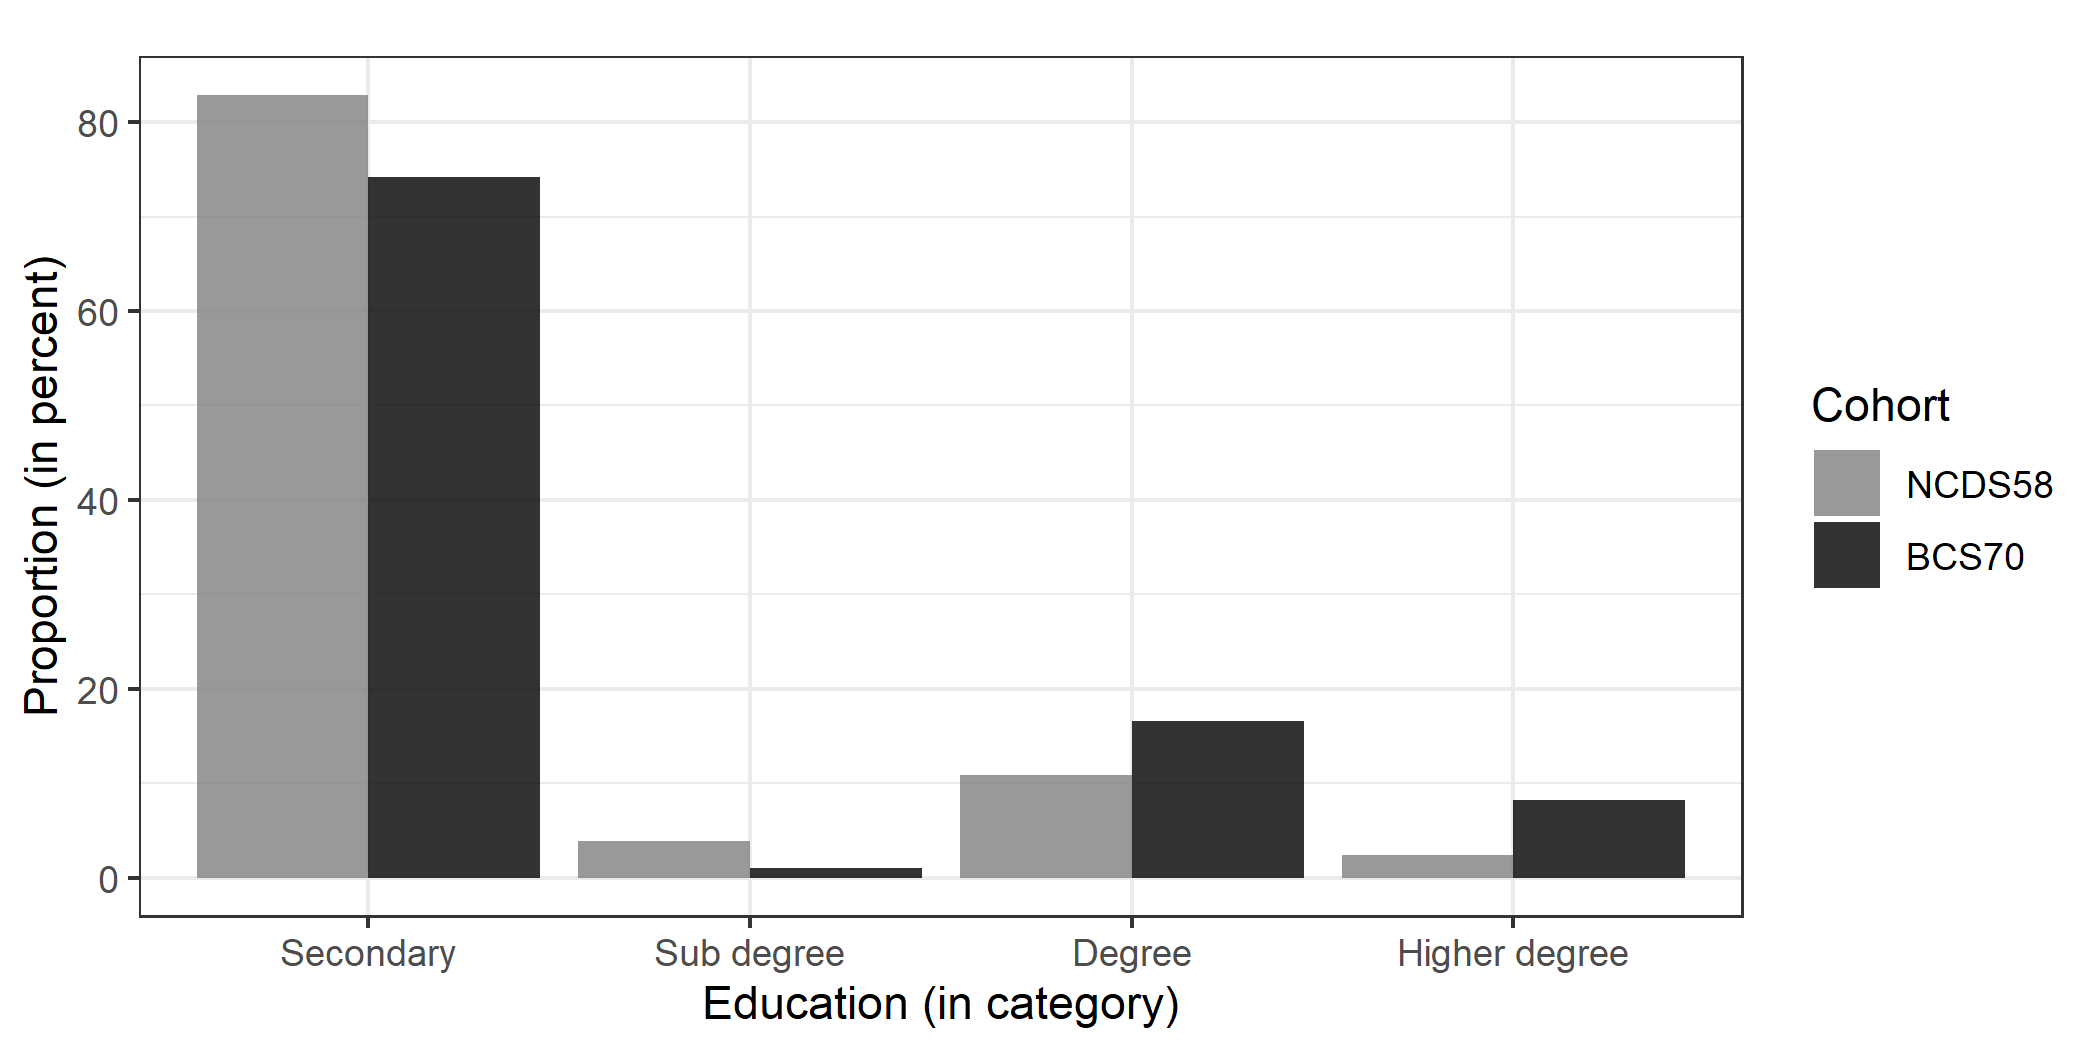
\includegraphics[width=\linewidth]{chap2/graphic/stat-educ-child-short.png}
	\vspace{-3em}
	\justify\singlespacing\footnotesize{\textit{Notes:} This figure presents the distribution of child education for the NCDS58 and BCS70 cohorts. Education corresponds to the highest academic qualification obtained by the child. Education levels are grouped into four categories for readability.}
\end{figure}

\begin{figure}[!htb]
    \centering
    \caption{Parental education distribution}
    \label{chap2-fig:stat-educ-parents}
    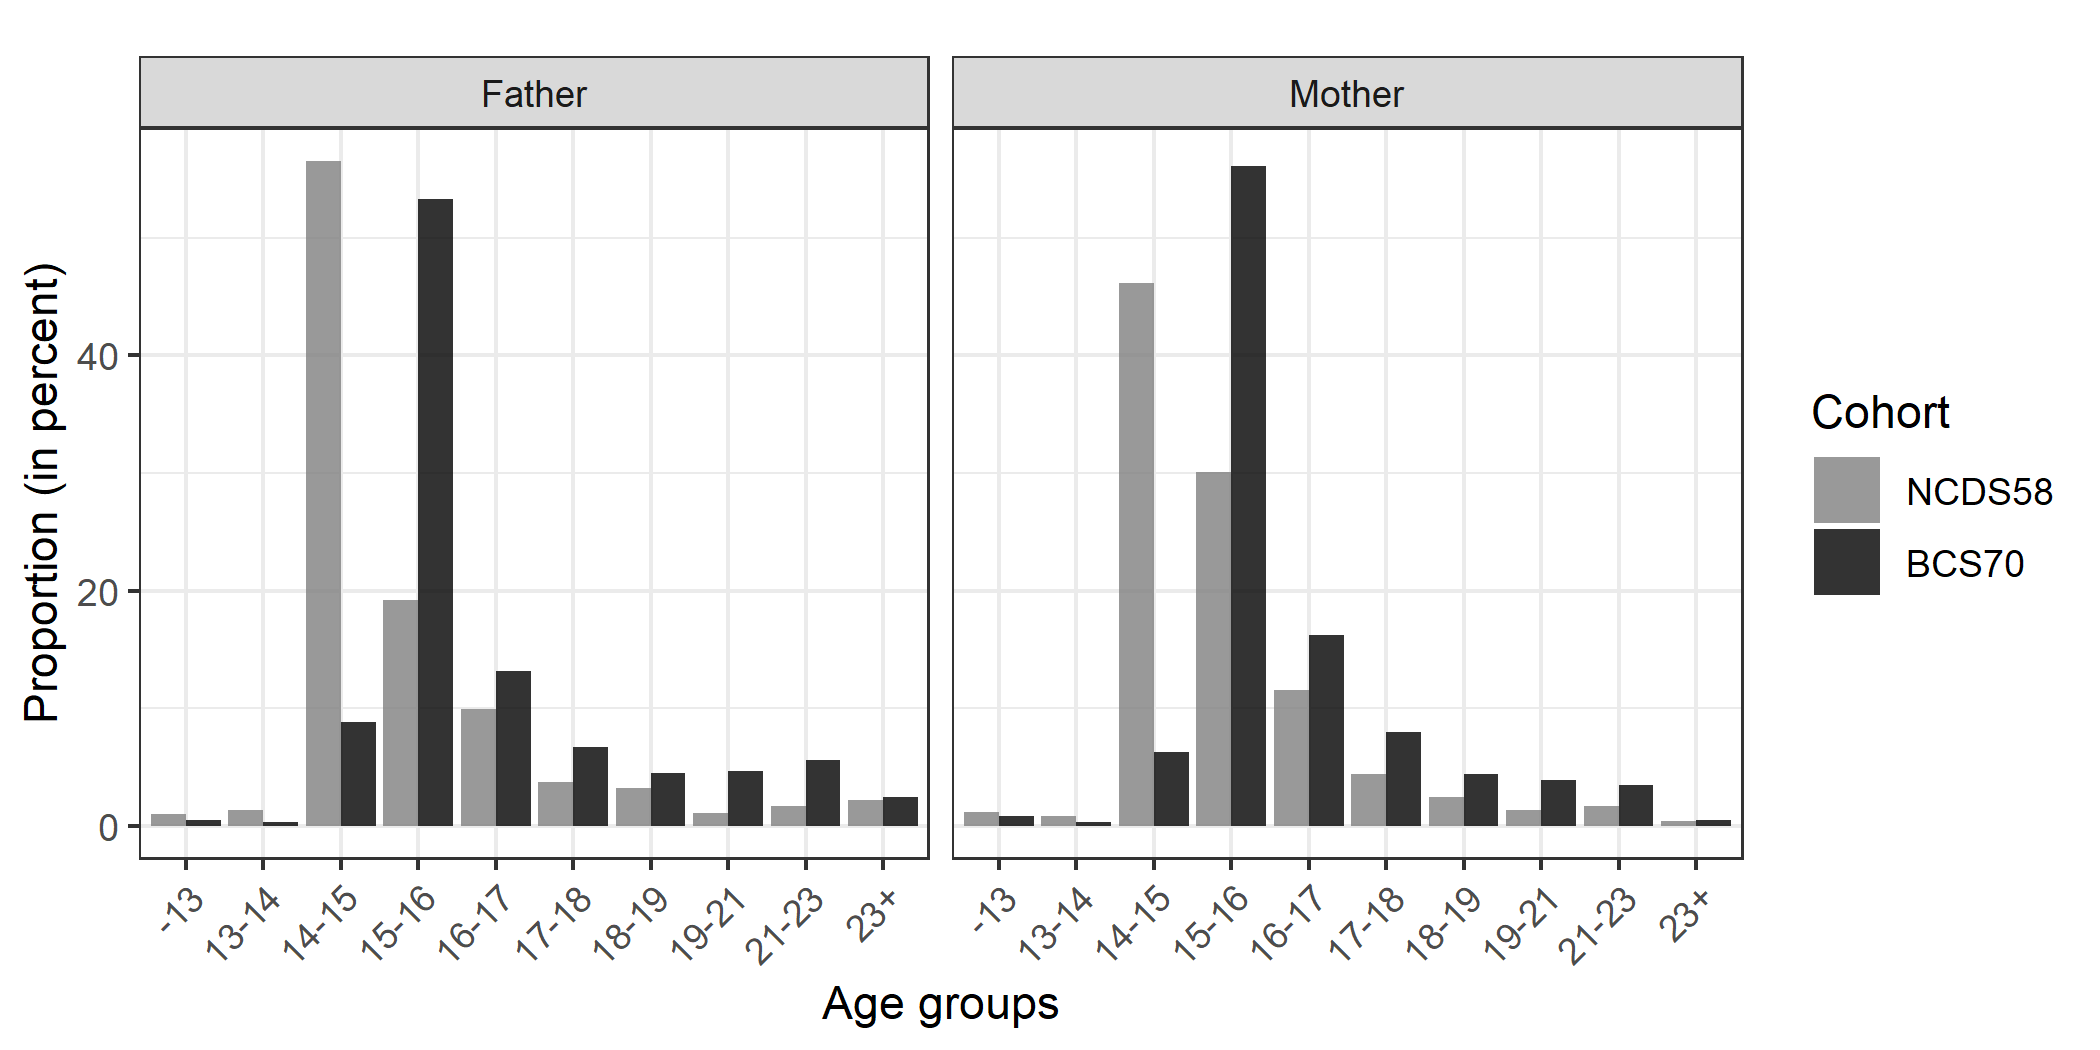
\includegraphics[width=\linewidth]{chap2/graphic/stat-educ-parents.png}
	\vspace{-3em}
	\justify\singlespacing\footnotesize{\textit{Notes:} This figure presents the distribution of parents' education for the NCDS58 and BCS70 cohorts. Parental education refers to the age at which parents left school that is used as a proxy. Education levels at the bottom and top are grouped for readability.}
\end{figure}

\textbf{Occupational structure.} In the data, occupations are reported according to e ISCO-88 categories. In Figure \ref{chap2-fig:stat-occ} we grouped occupations in three broad categories in line with the polarization literature, while Figure \ref{chap2-fig:polarize-isco88-both} performs a similar exercise using the original ISCO-88 categories. Occupations are depicted in light gray for those we place in the low-paying category, in dark grey for those in the middling category, and in black for high-paying ones. Although there are differences within the three broad categories, a clear pattern emerges both when we consider young and mature individuals. The change has been particularly large for young individual's occupations, for whom the reduction in the share of middling jobs has been marked. 

\begin{figure}[!htb]
     \centering
     \caption{Change in the probability of being in each ISCO-88 occupation in both periods}
     \label{chap2-fig:polarize-isco88-both}
     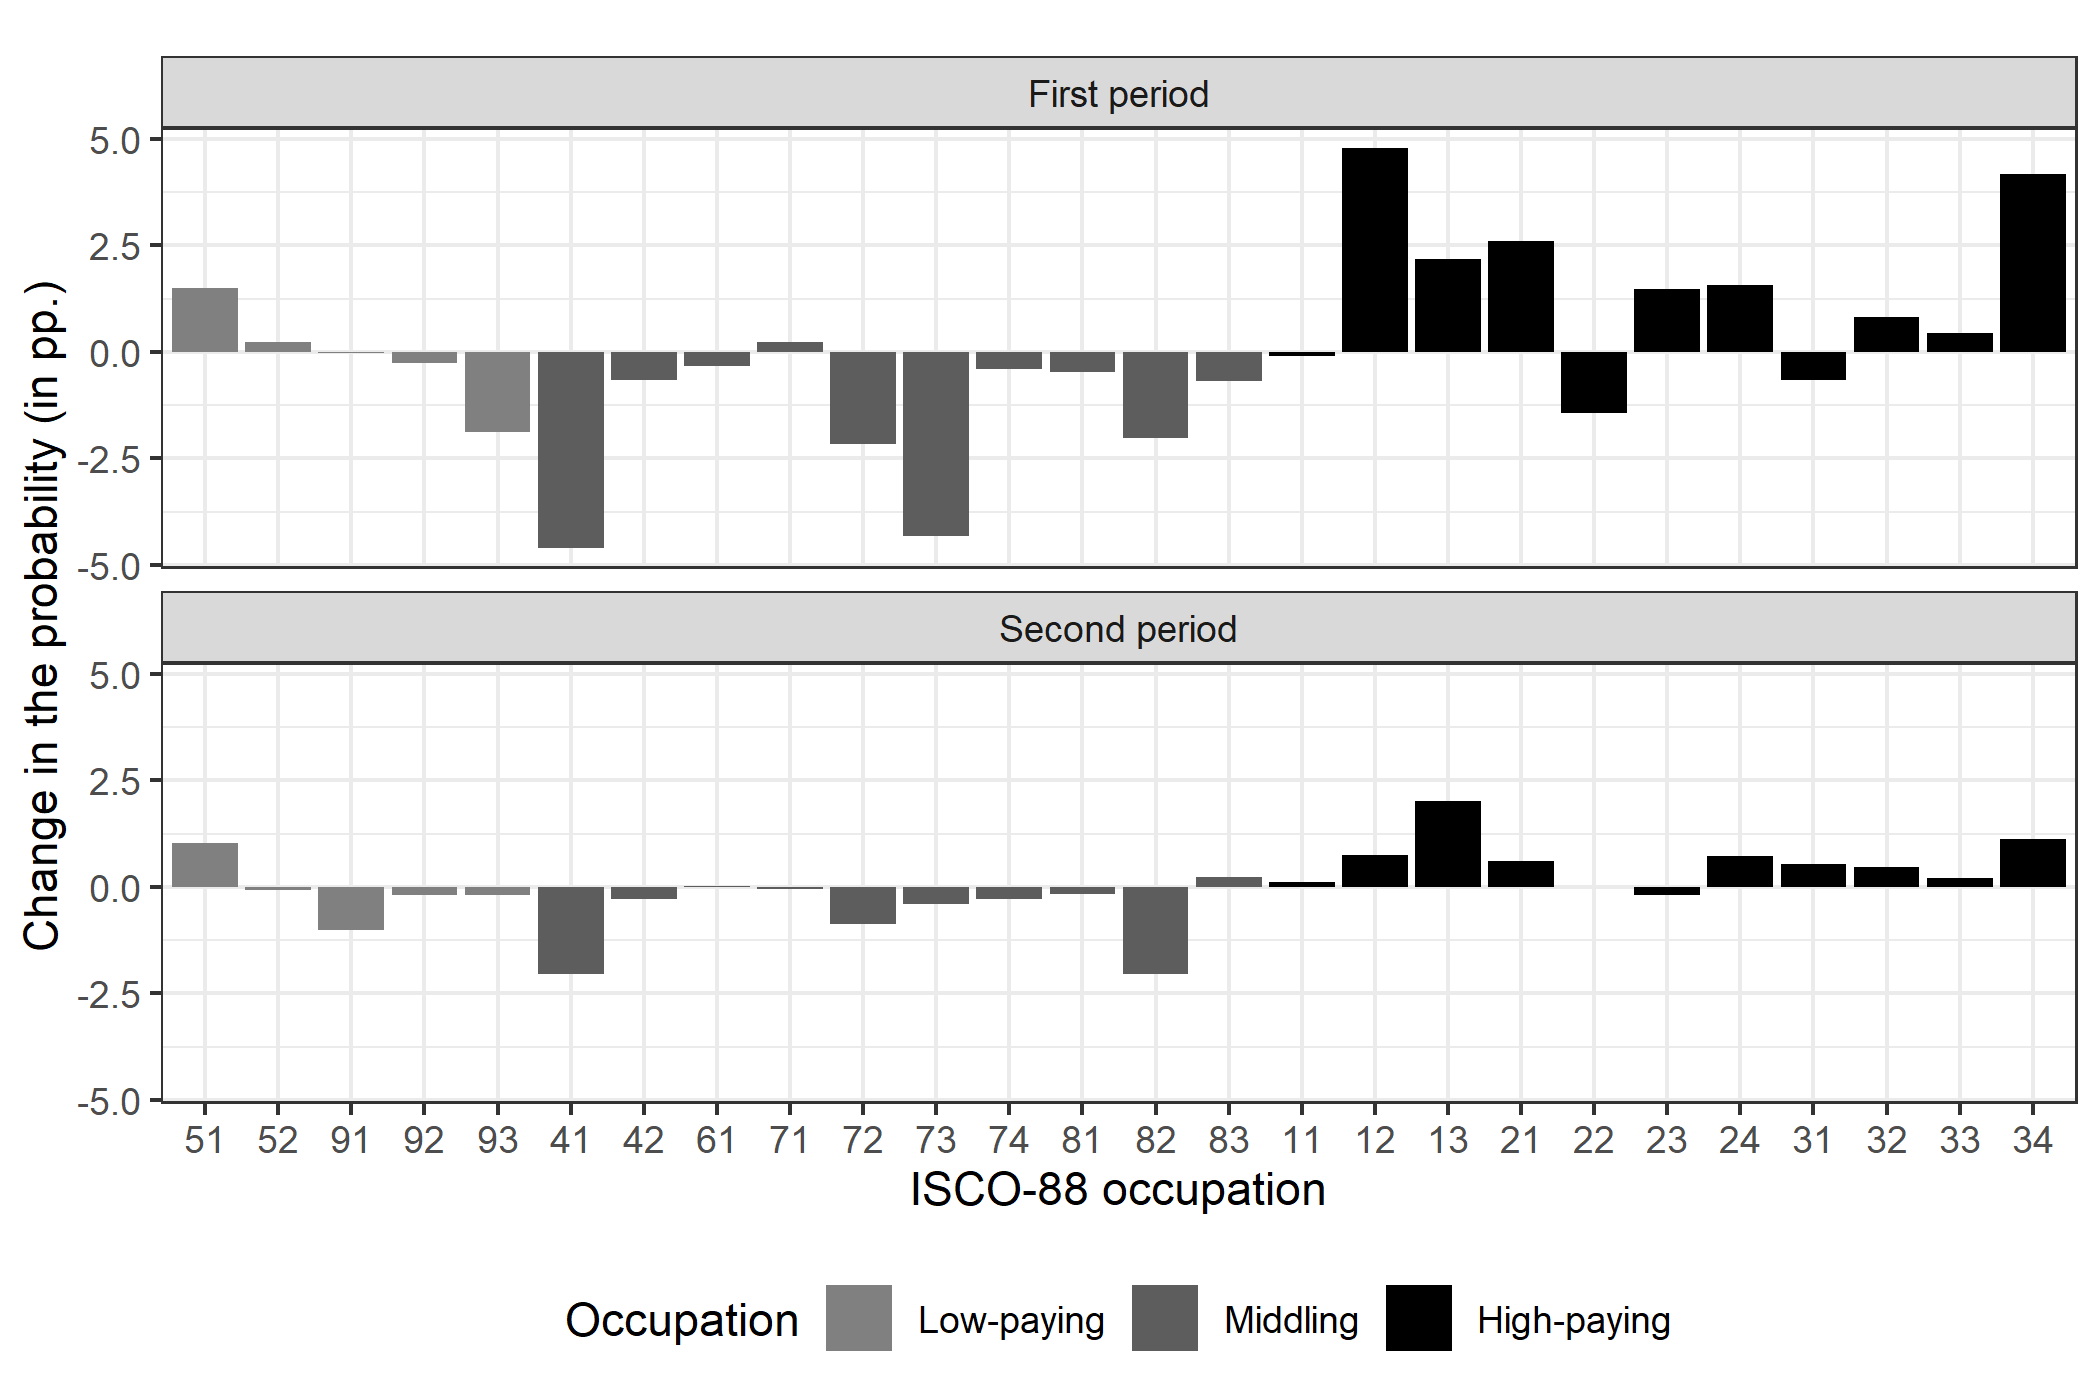
\includegraphics[width=\linewidth]{chap2/graphic/polarize-isco88-both.png}
 	\vspace{-3em}
 	\justify\singlespacing\footnotesize{\textit{Notes:} This figure presents the difference, expressed in percentage points, between the BCS70 and NCDS58 cohorts in terms of probability of being in each ISCO-88 occupation in both periods.}
\end{figure}


\subsubsection{The Labour Force Survey (1981-2012)}\label{chap2-app-data-LFS}

As a complementary dataset we use the Labor Force Survey (LFS). It is a random sampling of households living in the UK and collects data on labour market status and, since 1993, wages. The LFS was conducted every two years until 1983, then annually until 1992, and quarterly since then. It has the advantage of giving details on the occupation and industry in which individuals work, thus allowing us to take a snapshot of the structure of employment on a given year. The survey is intended to be representative of the whole population of the UK, and currently contains around 37,000 responding households in every quarter.

We use information from the LFS for the period 1981 to 2012, these being the years defined as the first-period for the older and the second-period for the younger cohorts. Initially the information is biannual, then annual from 1983 to 1992, and after that date we use data from the second quarter, as it is the one that most closely fits with the period over which annual interviews were conducted. The structure of the data allows us to define occupations in exactly the same way as for the cohort data and provides information on the region of employment.

Figure \ref{chap2-fig:lfs-national} shows the extent of job polarization at the national level using the LFS data. The share of middling jobs has declined by over 20 percentage points from 1981 to 2012. This reduction has been offset by an increase in the share of high-paying occupations by 16 percentage points over the same period, whereas the share of low-paying jobs has increased by 7 percentage points.
\begin{figure}[!htb]
    \centering
    \caption{Job polarization at the national level (The Labour Force Survey)}
    \label{chap2-fig:lfs-national}
    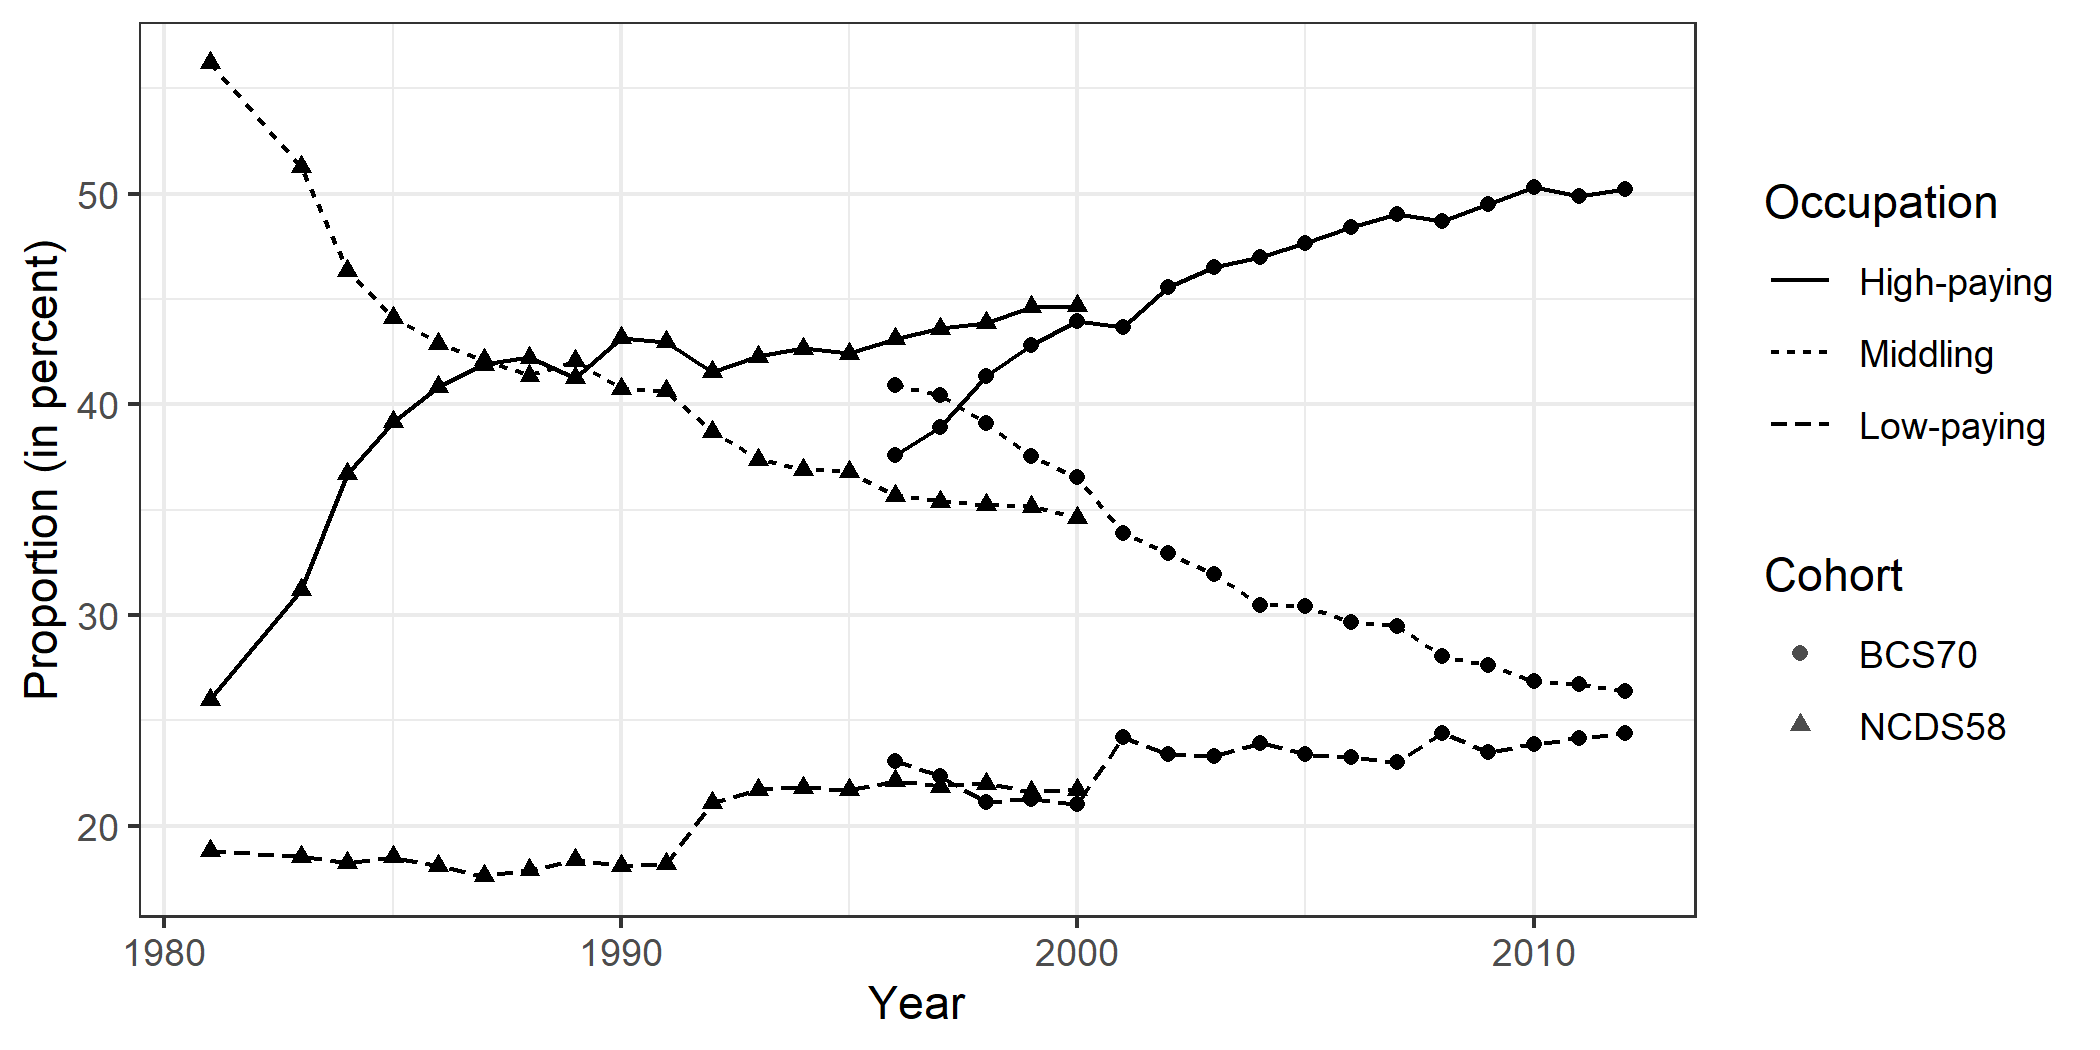
\includegraphics[width=\linewidth]{chap2/graphic/lfs-national.png}
	\vspace{-3em}
	\justify\singlespacing\footnotesize{\textit{Notes:} This figure presents the job polarization at the national level using the Labour Force Survey (LFS) data from 1981 to 2012. Curves represent the share of individuals in low-paying, middling, and high-paying occupations for the relevant age cohort in the LFS, i.e. from those born five years before to those born five years latter.}
\end{figure}

\begin{figure}[!htb]
    \centering
    \caption{Job polarization at the regional level over the lifecycle of both cohorts}
    \label{chap2-fig:lfs-regional}
    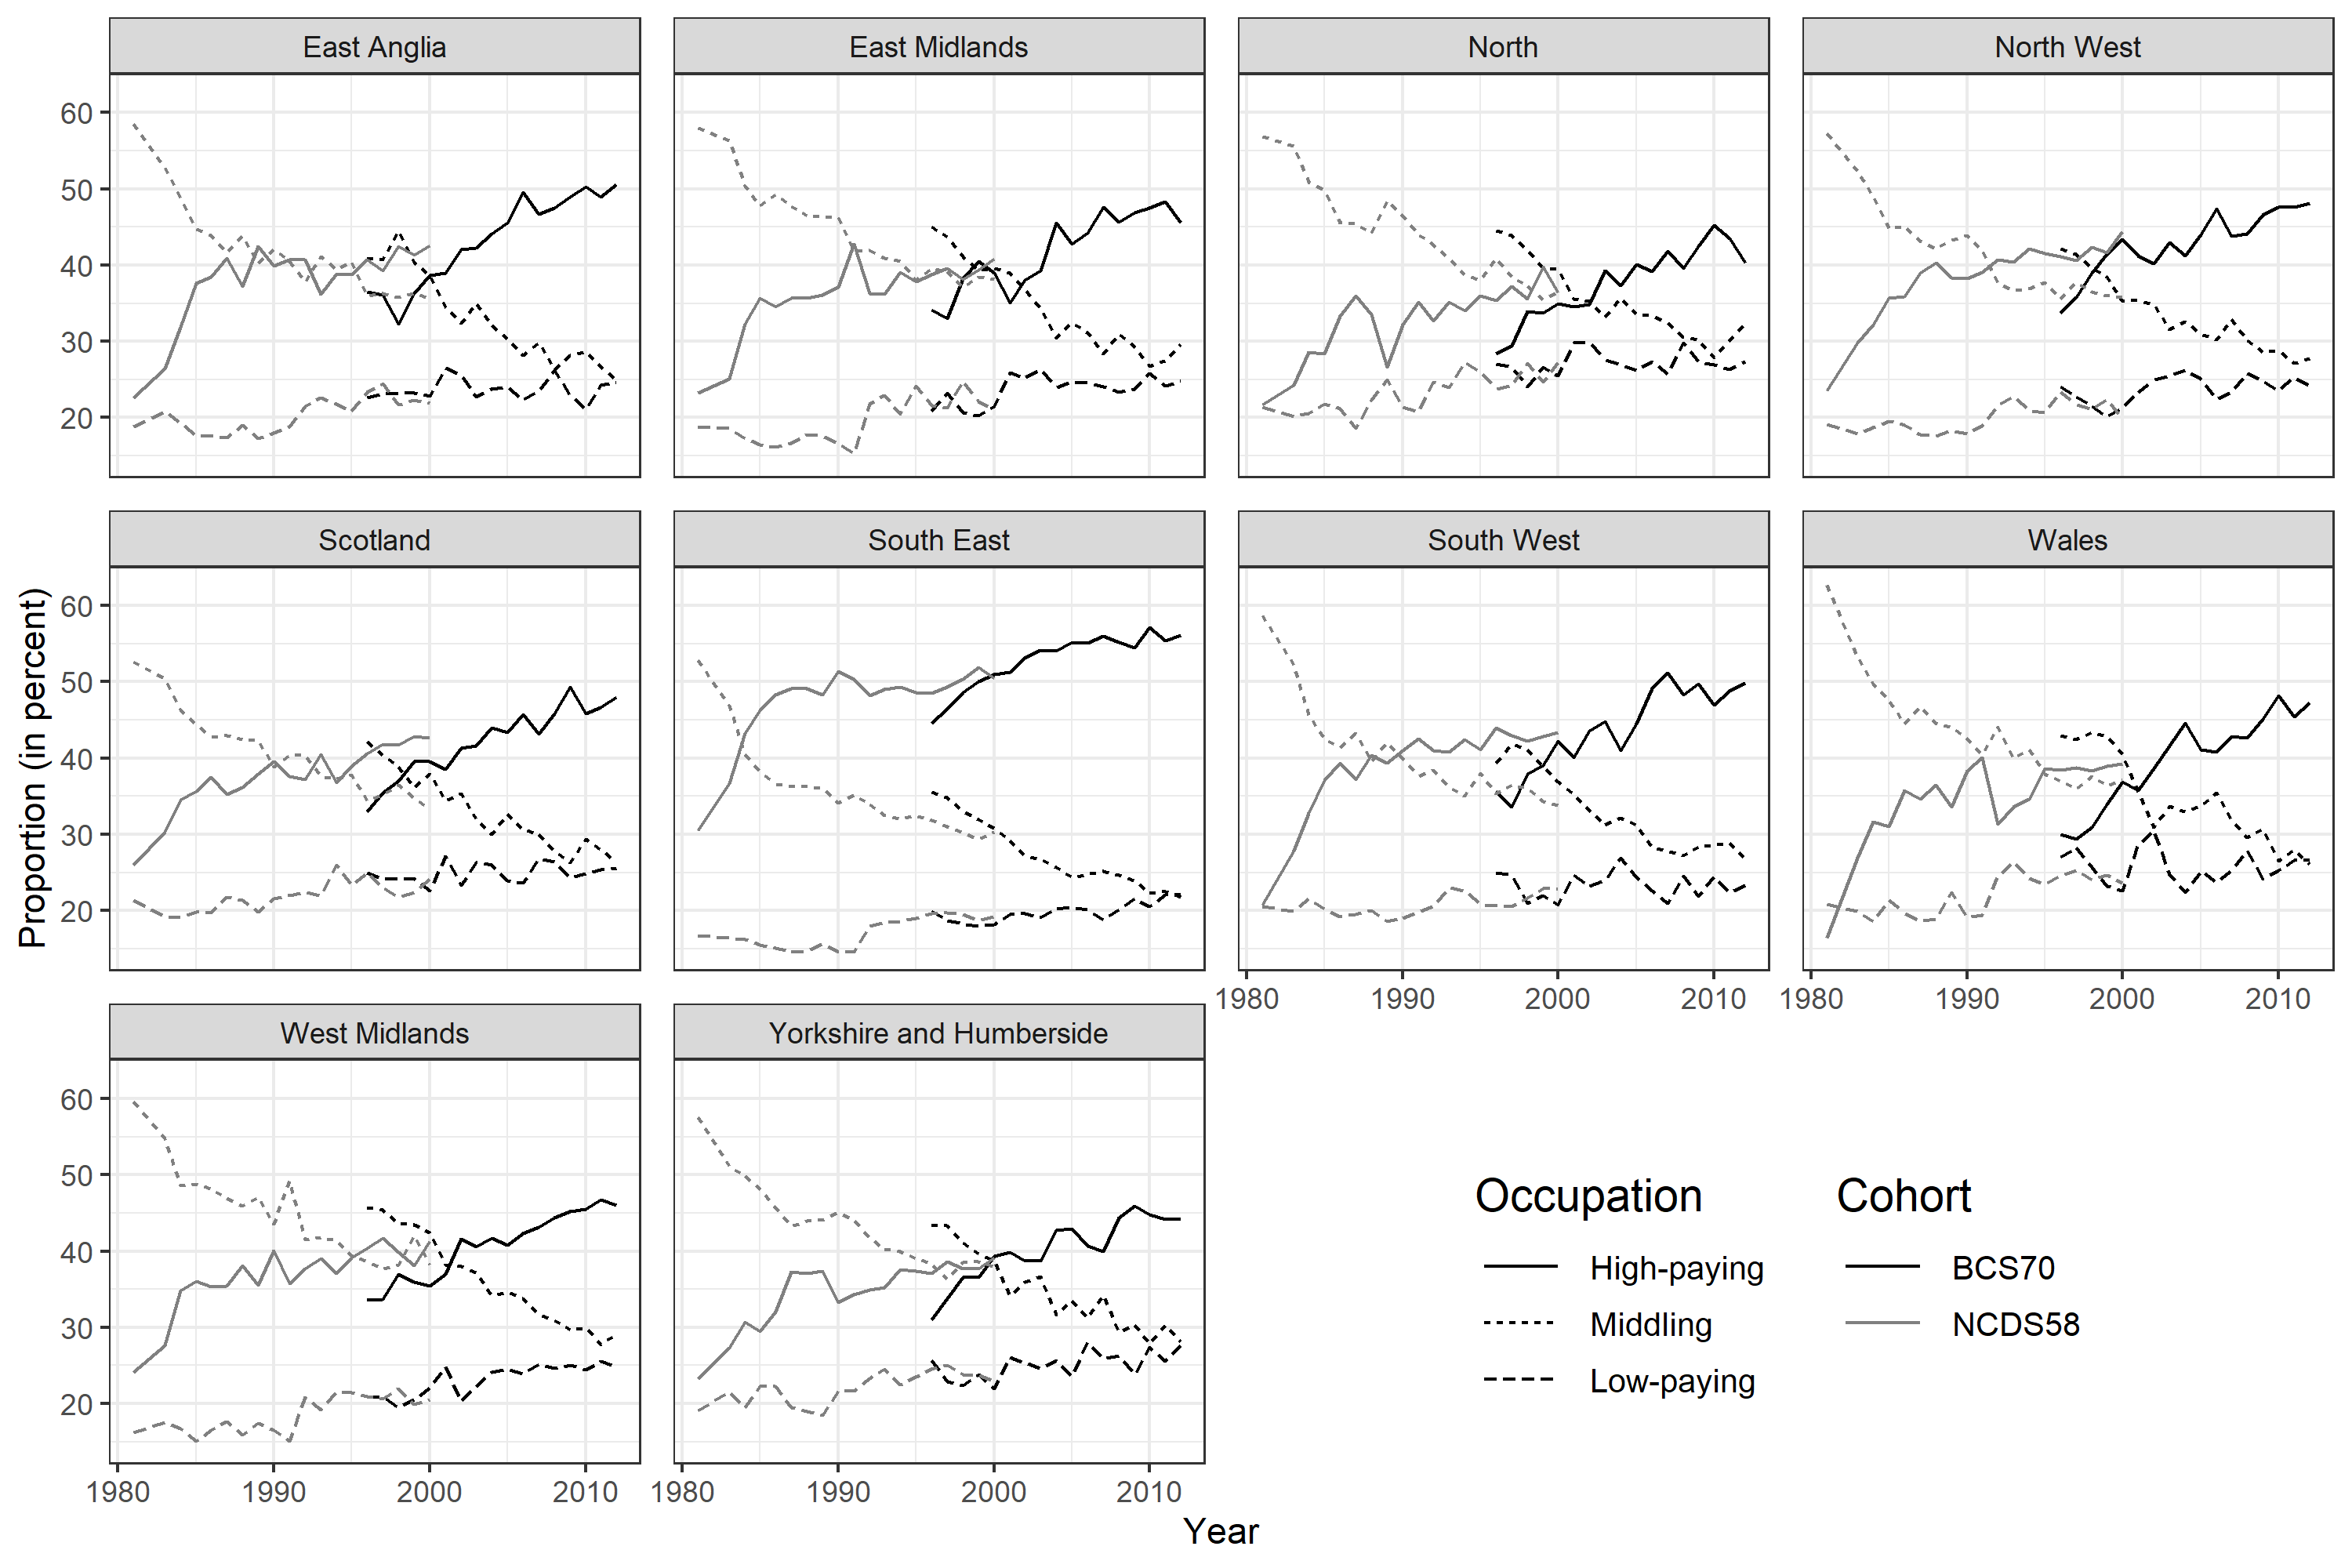
\includegraphics[width=\linewidth]{chap2/graphic/lfs-regional.png}
	\vspace{-3em}
	\justify\singlespacing\footnotesize{\textit{Notes:} This figure presents the job polarization at the regional level using the Labour Force Survey (LFS) data from 1981 to 2012. Curves represent the share of individuals in out-of-work, low-paying, middling, and high-paying occupations for the relevant age cohort in the LFS, i.e. from those born five years before to those born five years latter.}
\end{figure}

\subsubsection{Occupational classification}\label{chap2-app-data-classification}

Table \ref{chap2-tab:data-isco88} describes the classification of occupations that we use, providing an overview of ISCO-88 occupation codes along with the routine task intensities from \cite{Goos2014Explaining} and \cite{Mahutga2018Job}.
\begin{table}[!htb]
    \centering
    \begin{threeparttable}
        \caption{Overview of ISCO-88 occupation codes and routine task intensity}
        \label{chap2-tab:data-isco88}
        
\begin{tabular}{rlrr}
\toprule
\multicolumn{1}{c}{} & \multicolumn{1}{c}{} & \multicolumn{2}{c}{RTI} \\
\cmidrule(l{3pt}r{3pt}){3-4}
\textbf{Code} & \textbf{Occupation} & \textbf{GMS} & \textbf{LIS}\\
\midrule
\addlinespace[0.3em]
\multicolumn{4}{l}{\textbf{High-paying occupations}}\\
\hspace{1em}11 & Legislators and senior officials &  & -0.54\\
\hspace{1em}12 & Corporate managers & -0.75 & -0.62\\
\hspace{1em}13 & Managers of small enterprises & -1.52 & -1.41\\
\hspace{1em}21 & Physical, mathematical and engineering professionals & -0.82 & -0.70\\
\hspace{1em}22 & Life science and health professionals & -1.00 & -0.88\\
\hspace{1em}23 & Teaching professionals &  & -1.43\\
\hspace{1em}24 & Other professionals & -0.73 & -0.61\\
\hspace{1em}31 & Physical, mathematical and engineering associate professionals & -0.40 & -0.27\\
\hspace{1em}32 & Life science and health associate professionals & -0.33 & -0.20\\
\hspace{1em}33 & Teaching associate professionals &  & -1.33\\
\hspace{1em}34 & Other associate professionals & -0.44 & -0.32\\
\addlinespace[0.3em]
\multicolumn{4}{l}{\textbf{Middling occupations}}\\
\hspace{1em}41 & Office clerks & 2.24 & 2.39\\
\hspace{1em}42 & Customer service clerks & 1.41 & 1.55\\
\hspace{1em}61 & Skilled agricultural and fishery workers &  & 0.16\\
\hspace{1em}71 & Extraction and building trades workers & -0.19 & -0.06\\
\hspace{1em}72 & Metal, machinery and related trade work & 0.46 & 0.59\\
\hspace{1em}73 & Precision, handicraft, craft printing and related trade workers & 1.59 & 1.73\\
\hspace{1em}74 & Other craft and related trade workers & 1.24 & 1.38\\
\hspace{1em}81 & Stationary plant and related operators & 0.32 & 0.46\\
\hspace{1em}82 & Machine operators and assemblers & 0.49 & 0.63\\
\hspace{1em}83 & Drivers and mobile plant operators & -1.50 & -1.38\\
\addlinespace[0.3em]
\multicolumn{4}{l}{\textbf{Low-paying occupations}}\\
\hspace{1em}51 & Personal and protective service workers & -0.60 & -0.47\\
\hspace{1em}52 & Models, salespersons and demonstrators & 0.05 & 0.18\\
\hspace{1em}91 & Sales and service elementary occupations & 0.03 & 0.16\\
\hspace{1em}92 & Agricultural, fishery and related labourers &  & 0.39\\
\hspace{1em}93 & Laborers in mining, construction, manufacturing and transport & 0.45 & 0.58\\
\bottomrule
\end{tabular}

        \begin{tablenotes}[flushleft]
            \footnotesize{\item \textit{Notes}: This table provides an overview of ISCO-88 occupation codes and their corresponding Routine Task Intensity (RTI) from \cite{Goos2014Explaining} (GMS) and \cite{Mahutga2018Job} (LIS). Occupation groups (high-paying, middling and low-paying) correspond to those from \cite{Goos2014Explaining}, except for occupations 11, 23, 34, 61 and 92 that were removed from their analysis. We add these missing occupations to categories according to closest occupations, hence, relying on the 1-digit ISCO-88 classification.}
        \end{tablenotes}
    \end{threeparttable}
\end{table}
Table \ref{chap2-tab:stat-cohper} displays the shares of the various activity status and occupational categories.
\begin{table}[!htb]
    \centering
    \caption{Summary statistics - Cohort data per period}
    \label{chap2-tab:stat-cohper}
    \begin{threeparttable}
        % \setlength{\tabcolsep}{3pt}
        
\begin{tabular}{lrrrrrrrr}
\toprule
\multicolumn{1}{c}{} & \multicolumn{4}{c}{NCDS58 - N = 6780} & \multicolumn{4}{c}{BCS70 - N = 7992} \\
\cmidrule(l{3pt}r{3pt}){2-5} \cmidrule(l{3pt}r{3pt}){6-9}
\multicolumn{1}{c}{} & \multicolumn{2}{c}{First period} & \multicolumn{2}{c}{Second period} & \multicolumn{2}{c}{First period} & \multicolumn{2}{c}{Second period} \\
\cmidrule(l{3pt}r{3pt}){2-3} \cmidrule(l{3pt}r{3pt}){4-5} \cmidrule(l{3pt}r{3pt}){6-7} \cmidrule(l{3pt}r{3pt}){8-9}
Variable & Mean & SD & Mean & SD & Mean & SD & Mean & SD\\
\midrule
Activity - Employee & 0.74 & 0.44 & 0.74 & 0.44 & 0.78 & 0.42 & 0.72 & 0.45\\
Activity - Self-employed & 0.05 & 0.21 & 0.12 & 0.33 & 0.06 & 0.24 & 0.14 & 0.35\\
Activity - Unemployed & 0.05 & 0.23 & 0.02 & 0.14 & 0.02 & 0.16 & 0.02 & 0.14\\
Activity - in Education & 0.02 & 0.15 & 0.01 & 0.08 & 0.03 & 0.16 & 0.00 & 0.06\\
Activity - Inactive & 0.14 & 0.34 & 0.12 & 0.32 & 0.11 & 0.31 & 0.11 & 0.32\\
Occupation - High-paying & 0.24 & 0.42 & 0.39 & 0.49 & 0.36 & 0.48 & 0.44 & 0.50\\
Occupation - Middling & 0.41 & 0.49 & 0.28 & 0.45 & 0.33 & 0.47 & 0.24 & 0.43\\
Occupation - Low-paying & 0.14 & 0.35 & 0.19 & 0.39 & 0.15 & 0.36 & 0.18 & 0.39\\
Occupation - Out-of-work & 0.19 & 0.39 & 0.14 & 0.34 & 0.13 & 0.34 & 0.14 & 0.34\\
Occupation - in Education & 0.02 & 0.15 & 0.01 & 0.08 & 0.03 & 0.16 & 0.00 & 0.06\\
Pay & 19.06 & 7.23 & 30.35 & 24.20 & 25.21 & 16.47 & 36.01 & 25.54\\
\bottomrule
\end{tabular}

        \begin{tablenotes}[flushleft]
            \footnotesize{\item \textit{Notes}: This table provides summary statistics for individual time-variant data from the BCS70 and NCDS58 according to the period.}
        \end{tablenotes}
    \end{threeparttable}
\end{table}
Table \ref{chap2-tab:stat-pay} reports the average weekly pay by occupation in the cohort data. Weekly pay is more concentrated for young individuals than for mature ones, as wages tend to grow faster with age for those in high-paying occupations. The table indicates that the average pay has increased for every type of occupation between both cohorts. The change across cohort of pay at age 42 is roughly the same for the three categories, lying between 14 and 15\%. In contrast, for young individuals, the change has been much larger for those in high-paying occupations (50\%) than for the other two groups (13 and 20\%, respectively, in low-paying and middling occupations).

\begin{table}[!htb]
    \centering
    \caption{Average weekly pay by occupation (in 1970£)}
    \label{chap2-tab:stat-pay}
    \begin{threeparttable}
        \setlength{\tabcolsep}{18pt}
        \begin{tabular}{l D{.}{.}{3.3} D{.}{.}{3.3} D{.}{.}{3.3} D{.}{.}{3.3}}
\toprule
\multicolumn{1}{c}{} & \multicolumn{2}{c}{First period} & \multicolumn{2}{c}{Second period} \\
\cmidrule(l{3pt}r{3pt}){2-3} \cmidrule(l{3pt}r{3pt}){4-5}
Occupation & \multicolumn{1}{c}{NCDS58} & \multicolumn{1}{c}{BCS70} & \multicolumn{1}{c}{NCDS58} & \multicolumn{1}{c}{BCS70}\\
\midrule
Low-paying & 17.05 & 19.35 & 17.75 & 20.25\\
 & (0.30) & (0.61) & (0.39) & (0.37)\\
Middling & 19.60 & 23.42 & 25.26 & 29.07\\
 & (0.16) & (0.34) & (0.45) & (0.39)\\
High-paying & 19.51 & 29.23 & 40.82 & 46.64\\
 & (0.17) & (0.40) & (0.64) & (0.55)\\
\bottomrule
\end{tabular}

        \begin{tablenotes}[flushleft]
            \footnotesize{\item \textit{Notes}: This table presents the average weekly pay, expressed in 1970£, in each first- and second-period occupations for the NCDS58 and BCS70 cohorts. Standard errors between parentheses. We exclude the very bottom and top of the pay distribution for each cohort, i.e. pay which are below £1 and above £300.}
        \end{tablenotes}
    \end{threeparttable}
\end{table}

Occupations are also characterized by different educational requirements. Note, however, that a comparison across the two cohorts is not straight forward as the overall educational attainment of the population has increased, as seen in Figure \ref{chap2-fig:stat-educ-child-short}. Because of these changes, Table \ref{chap2-tab:stat-educ} reports average education by occupation using the peer-inclusive downward-looking ranking. As well as our three employment categories we also report the educational attainment of those who are not in employment, splitting this category into those in full time education and the rest of those who are out-of-work (unemployed or not participating).\footnote{In our data, child education is time invariant because we consider the highest qualification ever obtained. Although some individuals may still appear in the occupational category full-time education, their educational level is the one they will obtain in the future.} When we do not split this category we find that average education is rather high, this being the combination of the low attainment of those not participating or unemployed and the high attainment of those still in education.

\begin{table}[!htb]
    \centering
    \caption{Average education by occupations}
    \label{chap2-tab:stat-educ}
    \begin{threeparttable}
        \setlength{\tabcolsep}{18pt}
        \begin{tabular}{l D{.}{.}{3.3} D{.}{.}{3.3} D{.}{.}{3.3} D{.}{.}{3.3}}
\toprule
\multicolumn{1}{c}{} & \multicolumn{2}{c}{First period} & \multicolumn{2}{c}{Second period} \\
\cmidrule(l{3pt}r{3pt}){2-3} \cmidrule(l{3pt}r{3pt}){4-5}
Occupation & \multicolumn{1}{c}{NCDS58} & \multicolumn{1}{c}{BCS70} & \multicolumn{1}{c}{NCDS58} & \multicolumn{1}{c}{BCS70}\\
\midrule
Out-of-work & 0.55 & 0.51 & 0.54 & 0.54\\
 & (0.01) & (0.01) & (0.01) & (0.01)\\
Education & 0.89 & 0.79 & 0.84 & 0.62\\
 & (0.01) & (0.01) & (0.03) & (0.05)\\
Low-paying & 0.54 & 0.52 & 0.52 & 0.51\\
 & (0.01) & (0.01) & (0.00) & (0.00)\\
Middling & 0.58 & 0.54 & 0.55 & 0.53\\
 & (0.00) & (0.00) & (0.00) & (0.00)\\
High-paying & 0.74 & 0.72 & 0.73 & 0.70\\
 & (0.01) & (0.00) & (0.00) & (0.00)\\
\bottomrule
\end{tabular}

        \begin{tablenotes}[flushleft]
            \footnotesize{\item \textit{Notes}: This table presents the average education, expressed in peer-inclusive downward-looking ranking, in each first- and second-period occupations for the NCDS58 and BCS70 cohorts. Standard errors between parentheses.}
        \end{tablenotes}
    \end{threeparttable}
\end{table}

\subsubsection{Structure of employment}\label{chap2-app-data-structure}

Table \ref{chap2-tab:proba-group4-abs} presents the probability to be in each occupation at both periods, for both cohorts. The first-period probabilities indicate that BCS70-cohort individuals are about 7.9 pp. less likely to start in middling occupations, while they are about 12.4 pp. more likely to start their careers in a high-paying occupation. The probabilities with those in education in a separate category, hence not included in out-of-work, are reported in Table \ref{chap2-tab:proba-group5-abs}. Table \ref{chap2-tab:proba-group5-cdt-short} provides the probability of being in each second-period occupation conditional on the first-period occupation, isolating those in-education from the out-of-work. 

\begin{table}[!htb]
    \centering
    \caption{Probability of being in each occupation at both periods, for both cohorts (in percent)}
    \label{chap2-tab:proba-group4-abs}
    \begin{threeparttable}
        \setlength{\tabcolsep}{10pt}
        
\begin{tabular}{lrrrrrr}
\toprule
\multicolumn{1}{c}{} & \multicolumn{3}{c}{First period} & \multicolumn{3}{c}{Second period} \\
\cmidrule(l{3pt}r{3pt}){2-4} \cmidrule(l{3pt}r{3pt}){5-7}
Occupation & BCS70 & NCDS58 & $\Delta$ & BCS70 & NCDS58 & $\Delta$\\
\midrule
Out-of-work & 16.2 & 21.3 & -5.1 & 13.9 & 14.4 & -0.4\\
Low-paying & 15.2 & 14.0 & 1.2 & 18.4 & 19.1 & -0.7\\
Middling & 33.1 & 41.2 & -8.1 & 23.8 & 28.0 & -4.2\\
High-paying & 35.6 & 23.6 & 12.1 & 43.9 & 38.5 & 5.4\\
\bottomrule
\end{tabular}

        \begin{tablenotes}[flushleft]
            \footnotesize{\item \textit{Notes}: This table shows the probability, expressed in percent, of being in each first- and second-period occupation for the BCS70 and NCDS58 cohorts. Differences between both cohorts, expressed in percentage points, are reported in the last column of both periods.}
        \end{tablenotes}
    \end{threeparttable}
\end{table}

\begin{table}[!htb]
     \centering
     \caption{Probability to be in each occupation at both periods, isolating those in-education (in percent)}
     \label{chap2-tab:proba-group5-abs}
    \begin{threeparttable}
        % \small
        \setlength{\tabcolsep}{10pt}
        
\begin{tabular}{lrrrrrr}
\toprule
\multicolumn{1}{c}{} & \multicolumn{3}{c}{First period} & \multicolumn{3}{c}{Second period} \\
\cmidrule(l{3pt}r{3pt}){2-4} \cmidrule(l{3pt}r{3pt}){5-7}
Occupation & BCS70 & NCDS58 & $\Delta$ & BCS70 & NCDS58 & $\Delta$\\
\midrule
Out-of-work & 13.5 & 19.1 & -5.6 & 13.6 & 13.7 & -0.1\\
in-Education & 2.7 & 2.2 & 0.5 & 0.3 & 0.6 & -0.3\\
Low-paying & 15.2 & 14.0 & 1.2 & 18.4 & 19.1 & -0.7\\
Middling & 33.1 & 41.2 & -8.1 & 23.8 & 28.0 & -4.2\\
High-paying & 35.6 & 23.6 & 12.1 & 43.9 & 38.5 & 5.4\\
\bottomrule
\end{tabular}

        \begin{tablenotes}[flushleft]
            \footnotesize{\item \textit{Notes}: This table shows the probability, expressed in percent, of being in each first- and second-period occupation for the BCS70 and NCDS58 cohorts. Differences between both cohorts, expressed in percentage points, are reported in the last column of both periods.}
        \end{tablenotes}
    \end{threeparttable}
\end{table}

\begin{table}[!htb]
    \centering
    \caption{Conditional probabilities of changing occupations during the career, isolating those in-education (in percent)}
    \label{chap2-tab:proba-group5-cdt-short}
    \resizebox{\textwidth}{!}{
    \begin{threeparttable}
        
\begin{tabular}{lrrrrrrrrrr}
\toprule
\multicolumn{1}{c}{} & \multicolumn{5}{c}{BCS70} & \multicolumn{5}{c}{NCDS58} \\
\cmidrule(l{3pt}r{3pt}){2-6} \cmidrule(l{3pt}r{3pt}){7-11}
Occupation & Out & Educ & Low & Mid & High & Out & Educ & Low & Mid & High\\
\midrule
Out-of-work & 37.0 & 0.7 & 28.3 & 15.2 & 18.9 & 28.5 & 0.9 & 26.9 & 22.1 & 21.6\\
in-Education & 14.0 & 0.5 & 10.7 & 11.2 & 63.7 & 10.7 & 0.0 & 5.3 & 8.0 & 76.0\\
Low-paying & 13.3 & 0.3 & 45.1 & 17.5 & 23.8 & 15.8 & 0.5 & 40.0 & 20.3 & 23.4\\
Middling & 10.2 & 0.3 & 13.8 & 44.9 & 30.8 & 9.9 & 0.5 & 15.4 & 43.4 & 30.8\\
High-paying & 8.0 & 0.2 & 8.2 & 11.0 & 72.6 & 7.6 & 0.8 & 8.1 & 12.3 & 71.2\\
\bottomrule
\end{tabular}

        \begin{tablenotes}[flushleft]
            \footnotesize{\item \textit{Notes}: Conditional probabilities with people in education included in out-of-work are reported in the paper, see table \ref{chap2-tab:proba-group4-cdt}.}
        \end{tablenotes}
    \end{threeparttable}
    }
\end{table}

Figure \ref{chap2-fig:polarize-isco88-pay-p3} presents the change in the frequencies of second period occupation according to the average weekly pay for the BCS70 cohort. 
Figure \ref{chap2-fig:polarize-rtiLIS-p3} displays the negative relationship between the probability of being in each second-period occupation according to its routine task intensity.

\begin{figure}[!htb]
    \centering
    \caption{Change in the probability of being in an occupation in the second period and average weekly pay}
    \label{chap2-fig:polarize-isco88-pay-p3}
    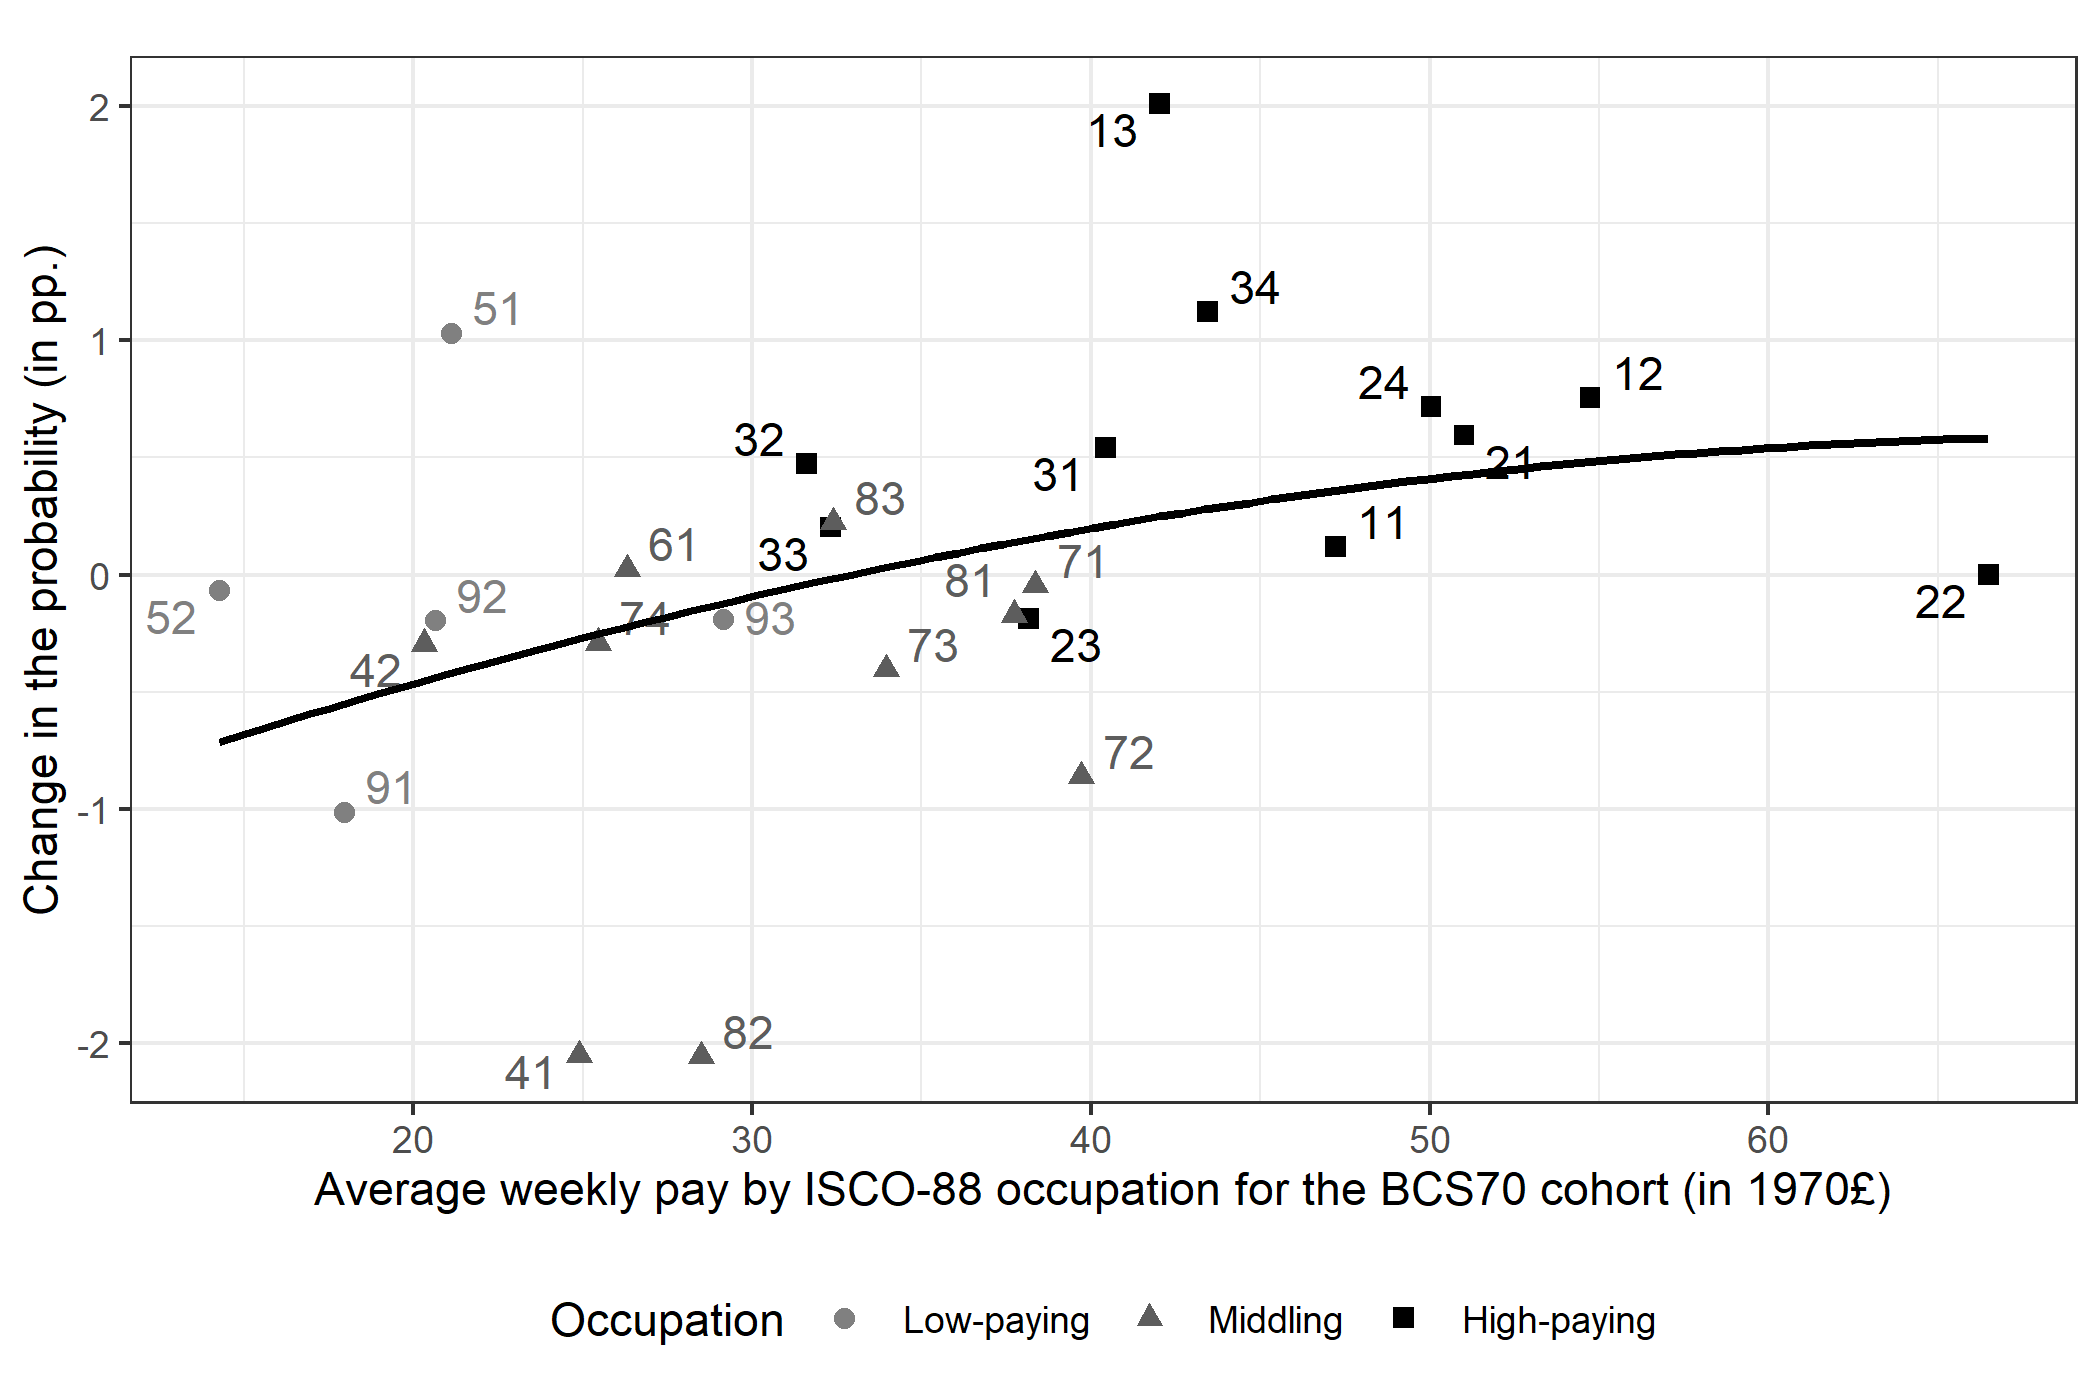
\includegraphics[width=\linewidth]{chap2/graphic/polarize-BCSpay-p3.png}
	\vspace{-3em}
	\justify\singlespacing\footnotesize{\textit{Notes:} This figure presents the positive relationship between the difference, expressed in percentage points, between the BCS70 and NCDS58 cohorts in terms of probability of being in each ISCO-88 occupation in second period and the average weekly pay, expressed in 1970£, in this occupation for the BCS70 cohort.}
\end{figure}

\begin{figure}[!htb]
    \centering
    \caption{Change in the probability of being in an occupation in the second period and routine task intensity}
    \label{chap2-fig:polarize-rtiLIS-p3}
    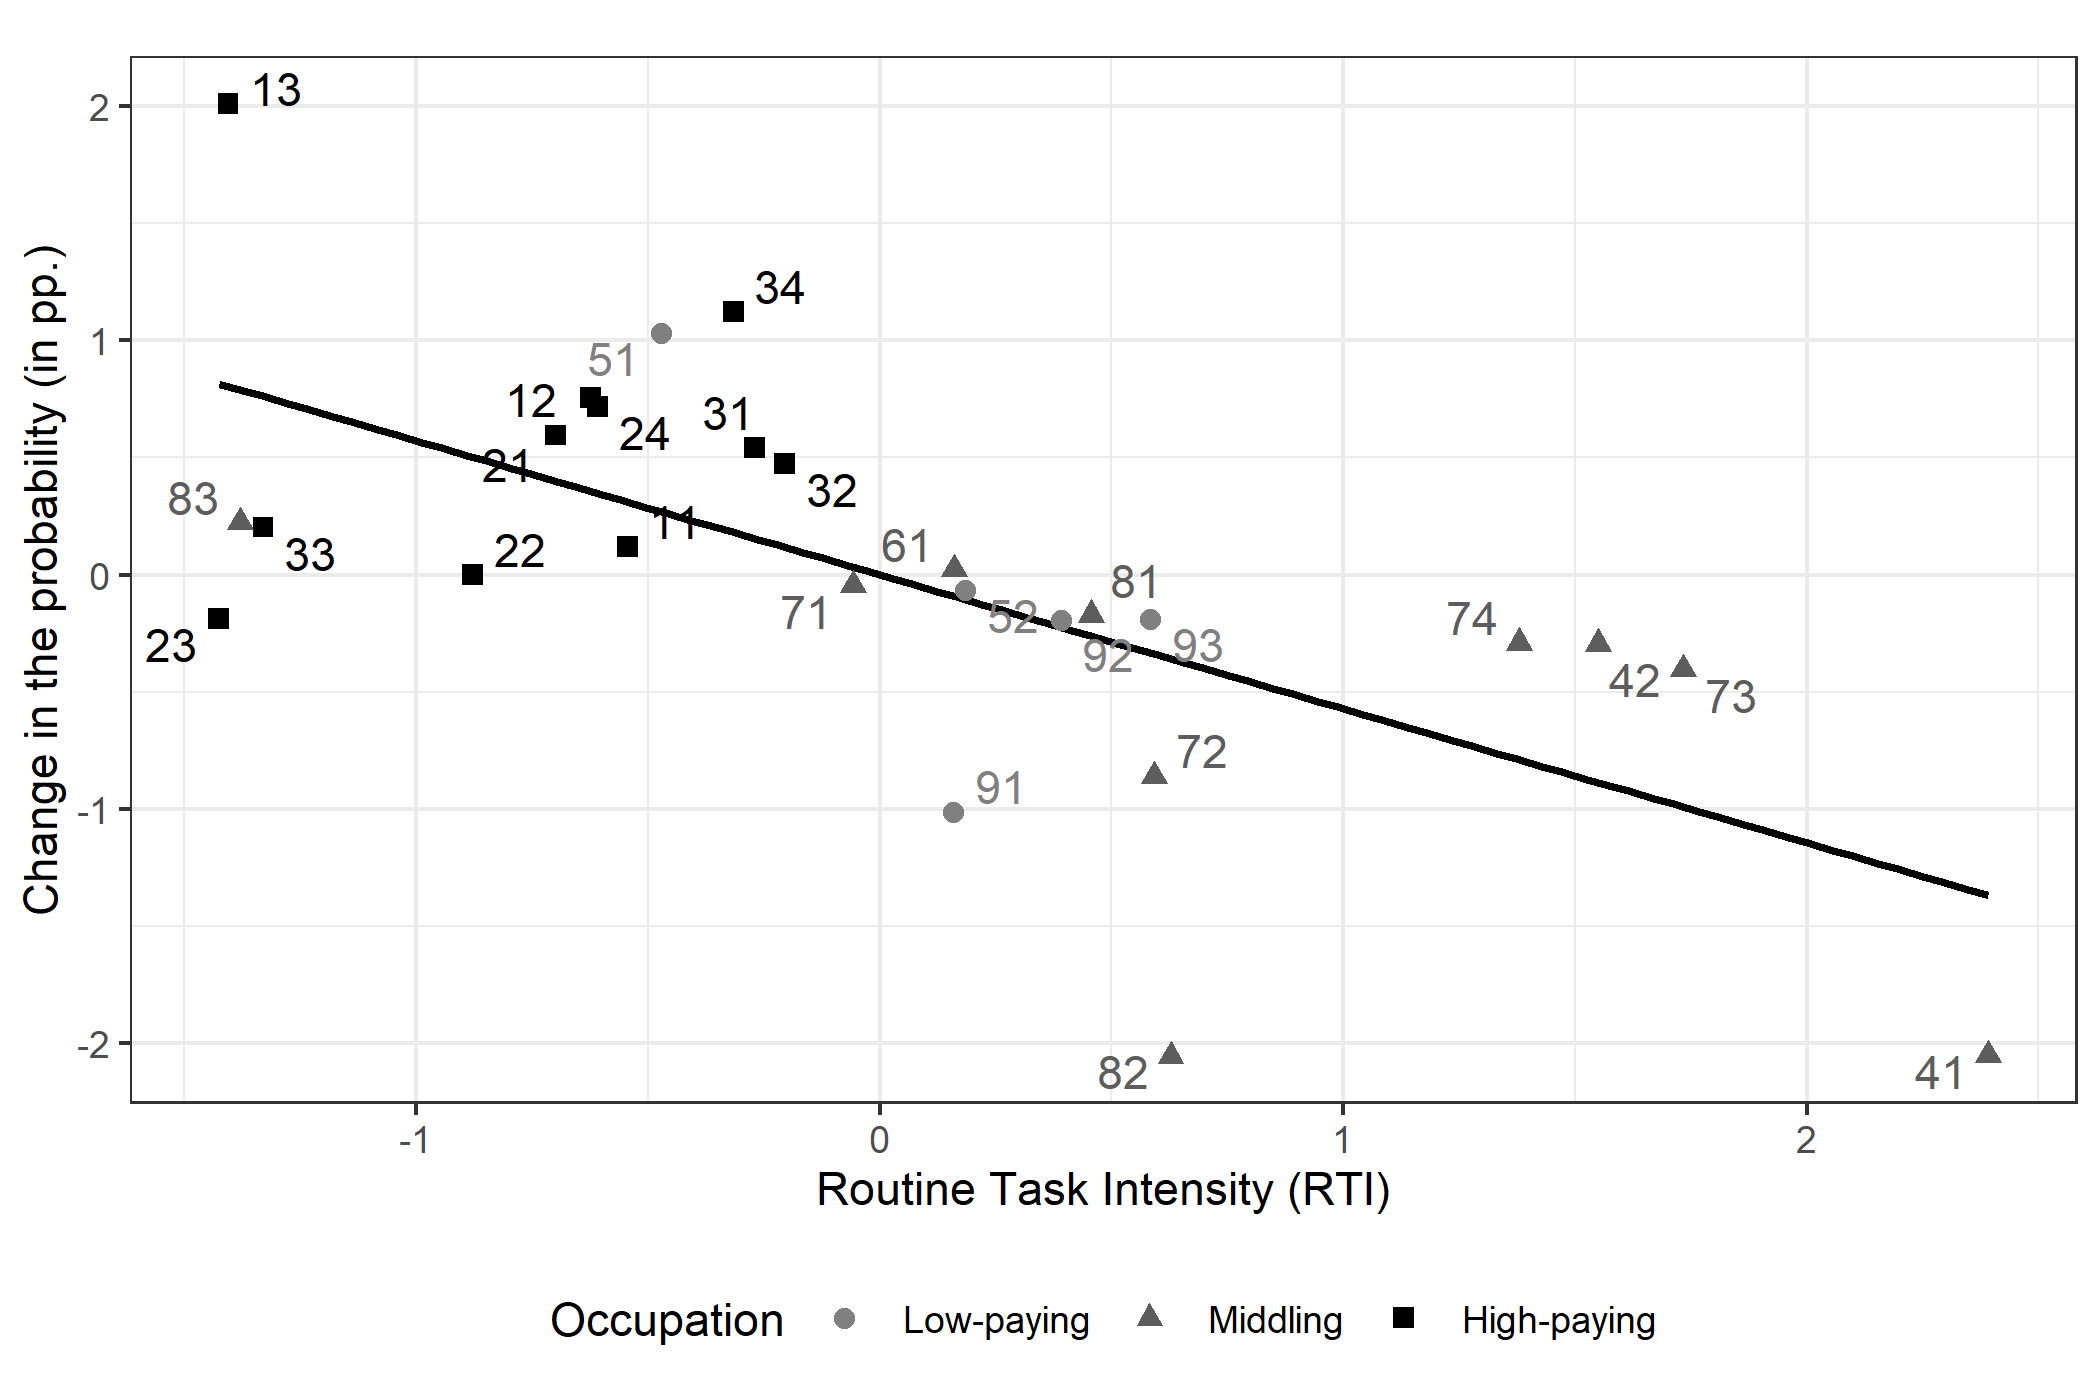
\includegraphics[width=\linewidth]{chap2/graphic/polarize-rtiLIS-p3.png}
	\vspace{-3em}
	\justify\singlespacing\footnotesize{\textit{Notes:} This figure shows the negative relationship between the difference, expressed in percentage points, between the BCS70 and NCDS58 cohorts in terms of probability of being in each ISCO-88 occupation in second period and the Routine Task Intensity (RTI) index from \cite{Mahutga2018Job}.}
\end{figure}

Lastly, Figure \ref{chap2-fig:lfs-change} reports the change in polarization in each of the regions obtained from the LFS.  

\begin{figure}[!htb]
    \centering
    \caption{Between-cohort change in the average share of total employment over the lifecycle of both cohorts (at the regional level)}
    \label{chap2-fig:lfs-change}
    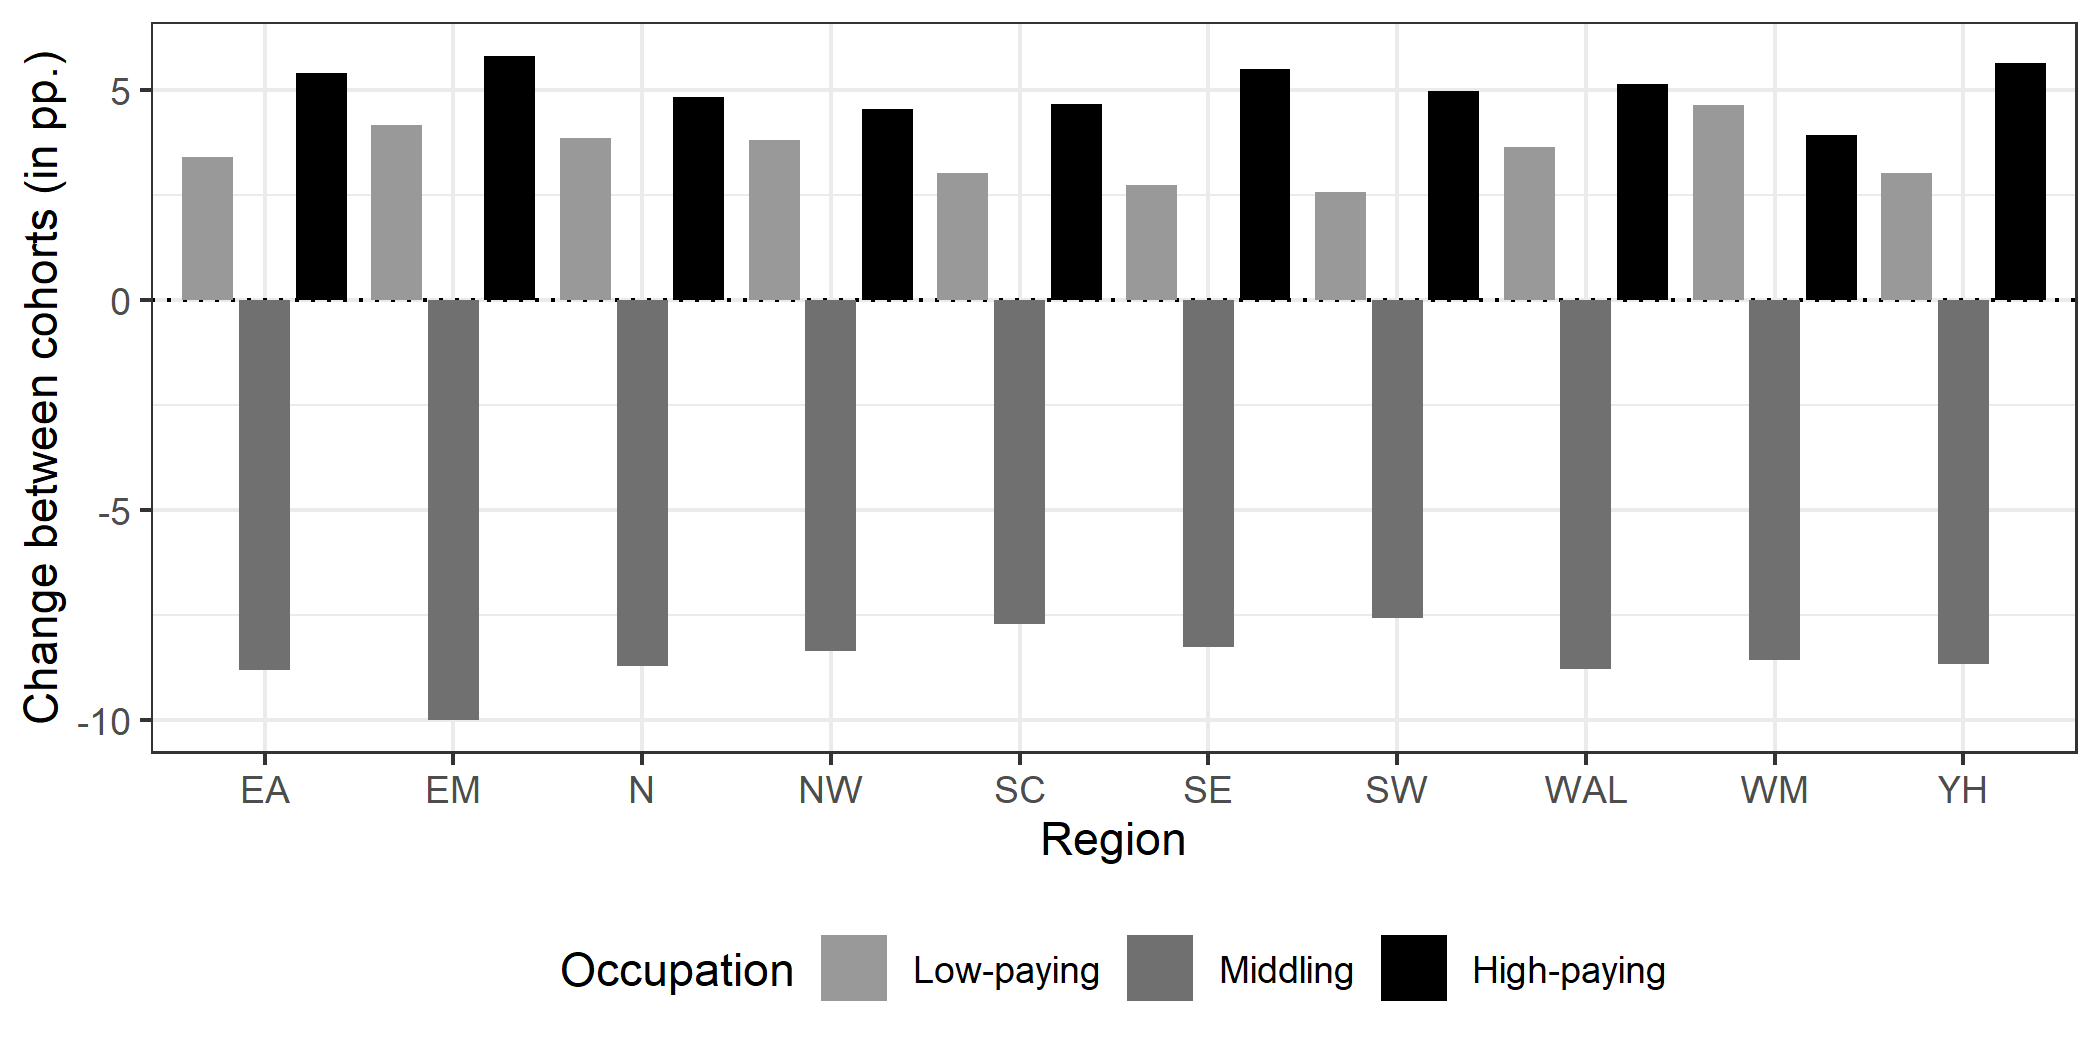
\includegraphics[width=\linewidth]{chap2/graphic/lfs-change.png}
	\vspace{-3em}
	\justify\singlespacing\footnotesize{\textit{Notes:} This figure presents the job polarization at the regional level using the Labour Force Survey data from 1981 to 2012.}
\end{figure}